\chapter{Introduction}
\label{chap:introduksjon}

Introduksjon
Nammo Gruppen er en teknologidreven romfart- og forsvarsvirksomhet som spesialiserer seg på høyytelsesløsninger. I porteføljen deres finnes blant annet rakettkastere, militær- og sportsammunisjon, rakettmotorer for militær- og romfartsbruk og miljøvennlige demilitariserings tjenester.



De ønsket seg en simulator for forbrenningen i sine fastoffraketter. Versjonen Nammo bruker i dag er en utdatert 2D versjon som er upraktisk og vanskelig å bruke. De kom derfor til NTNU på Gjøvik med en bachelor oppgave, for en bedre løsning. 


Formen på drivstoffet i fastoffraketter bestemmer hvor stor brennflaten er, som bestemmer kraften som blir produsert. Ved å kutte forskjellige former i brennstoffet kan en få varierende mengder kraft under forbrenningen. Vanligvis vil en ha mye kraft ved utskyting, for så å få mindre kraft for å opprettholde marsjhastighet.


Når Nammo skal utvikle en ny fastoffrakett starter de med en ønsket effektkurve, og må så finne en form for drivstoffet som gir den ønskede kurven. Dette gjøres gjennom eksperimentering, der de lager en modell for formen, beregner effektkurven og sammenligner den med den ønskelige kurven. De verktøyene de bruker til dette i dag er gamle, upraktiske og gir begrenset outputdata. Det er noen som har prøvd å gi ut noen alternativer, men ingen av disse er praktiske å bruke. Vi har da valgt å ta for oss en løsning som setter opp en god grunnleggende algoritme som kan bygges på videre for å få den ønsket funksjonalitet.


\section{Oppgavebeskrivelse}


Vi skal levere en programvaren som lar brukeren definere en 2D modell av drivstoffet og se hvordan effektkurven vil være umiddelbart, det skal også gi verdiene av kurven i tabellform.

Hovedfunksjonalitetene vil da være:
\begin{itemize}
    \item  Et 2D modelleringsverktøy
    \item Beregning av effektutvikling over tid
    \item  Presentasjon i graf- og tabellform
\end{itemize}


For å forklare litt bedre, har vi en rekke verdier som blir gitt av brukeren. Disse verdiene vil bli brukt til å skape den ønskede formen i brennstoffet. Disse formene er blant annet en form for stjerneform med  x antall armer. Programvaren kommer til å bruke disse parametrene til å finne hvordan denne formen kommer til å forandre seg under brenntiden. Dette blir gjort så brukeren kan få en oversikt over hvordan arealet til brennstoffet vil utvikle seg over tid. Dette gir brukeren en oversikt over hvordan rakettmotoren vil prestere. Denne beregningen består av en rekke linjestykker som vil forflytte seg en bestemt lengde som er bestemt av parametrene som har blitt gitt av brukeren. Denne informasjonen vil bli vist i to forskjellige former. Programvaren har en graf som viser effektutvikling over tid og en versjon som lager et Excel dokument og skriver tallverdiene til den.

\section{Hensikt}
Hensikten med dette prosjektet er å gjøre hverdagen til Nammo sine ansatte lettere. Når Nammo får en bestilling av raketter får de en graf over hvordan rakettmotoren skal prestere. Ut ifra denne grafen skal Nammo komme opp med et design av utskjæringen i brennstoffet. Denne løsningen vil gi utviklerne muligheten til å ta sin erfaring å raskt test hvordan en ønsket rakettmotor presterer og dermed øke effektiviteten til utviklere hos Nammo.

\section{Effektmål}
Vi løser oppgaven så Nammo kan raskere design nye rakettmotorer og gjøre hverdagen til de ansatte enklere. Denne programvare vil gi Nammo en fordel blant sine konkurrenter ettersom denne løsningen ikke eksisterer på markedet i dag.

\section{Resultatmål}
Med den ferdig utviklet programvaren ønsker vi å utvikle et system som:
Levere 4 hoved funksjonaliteter i en komplett løsning
	En visning av hvordan brennflaten ser ut
	En grafisk visning av presentasjonen til rakettmotoren
En numerisk visning i Excel
Muligheten til å definere formen på brennflaten

\section{Læringsmål}
Intensjonen med bachelor oppgaven er å gi oss en erfaring på større prosjekter over en lengre periode. Hvor vi planlegger, estimerer utvikler og levere helt alene. Når vi jobber i en gruppe vil vi måtte delegere oppgavene og ikke få den samme opplevelsen og læringsutbytte men vi håper begge lært noen av punktene under.

\begin{itemize}

   \item    Lære python og mange av de vanligste bibliotekene der, samt mer spesialiserte biblioteker rettet mot 2D modellering.
   
   \item    Bedre innsikt i systemplanleggingsprosessen og spesifikt gjennomføring av denne planen, med hvilke avvik og endringer som vil blir nødvendige.
   
   \item    Scrum systemutviklingsmodellen, og gjennom den bli flinkere å estimere tid- og resurssbruk i forbindelse med programvareutvikling.
   
   \item    2D modellering med implisitte flater, med de matematiske og programmatiske utfordringer det krever.
   
   \item    Lære Latex formatering for å skape rene, profesjonelle og strukturerte dokumenter.
   
\end{itemize}



 

I tillegg til disse punktene må begge lære og forstå  hvordan jobbe på en strukturert måte og sammen med evnen til å til reflektere arbeid som har blitt gjort. Arbeidet som blir gjort skal bli dokumentert og presentert på en vitenskapelig måte med tanke på hvordan innvirkning dette kan ha på individer og fagfeltet som en helhet.

\section{Målgruppe}
\subsection{Målgruppe for produktet}
Målgruppen for dette prosjektet vil være Nammo is rakett utviklingsavdeling. Programmet skal kjøres på en vanlig jobb laptop, det er derfor viktig at programmet krever for mye minne.
Programmet kommer til å blir brukt hyppig og krever et godt GUI som ikke krever en læringskurve for de som har minimal til ingen IT kunnskaper.


\subsection{Målgruppe for rapporten}
Hovedmålgruppen for rapporten er alle involverte i prosjektet, ansatte hos Nammo, veileder, fremtidige arbeidsgivere eller studenter og utviklere. Denne rapporten gir leseren en innsikt i hvordan vi har løst oppgaven gitt av Nammo og hvordan vi har valgt å utvikle programmet. Denne oppgaven kan være nyttig til andre studenter eller utviklere som et læringsverktøy for fremtidige bachelor rapporter eller private student prosjekter. Oppgaven forventer at leseren har grunnleggende datakunnskaper og er skrevet med tanke på dette. Rapporten er skrevet på norsk fordi dette er vårt morsmål. Vi valgte vårt morsmål fordi vi følte at det ville gi et bedre resultat og mindre tid og energi ville gå i rettskriving og setningsoppbygging, så vi kunne fokusere på ting vi mener trenger med tid selv om dette gjør at oppgave er tilgjengelig for en mindre målgruppe.

\section{Prosjektorganisasjon}
 \textbf{Martin Spongsveen} Hadde oppgaver som kontaktperson med Nammo, som inneholdt 
organisering av møter og forbindelse angående uklarheter. I tillegg vil han hovedsakelig jobbe med oppgaver som ikke krevde dype matematiske kunnskaper.\\

 \textbf{Jon Anders Sylvarnes} Oppgave var å jobbe med den grunnleggende algoritmen som
håndterer forflytningen.\\

 \textbf{Ivar Farup} - Veileder Som veileder er Ivar personen vi går til med spørsmål og problemer vi 
møter på under utviklingen eller med rapportskriving. Han vil gi oss råd om arbeidsprosessen i tillegg til tilbakemeldinger på vårt arbeid.\\
\graphicspath{ {Pictures\Bachelor} }
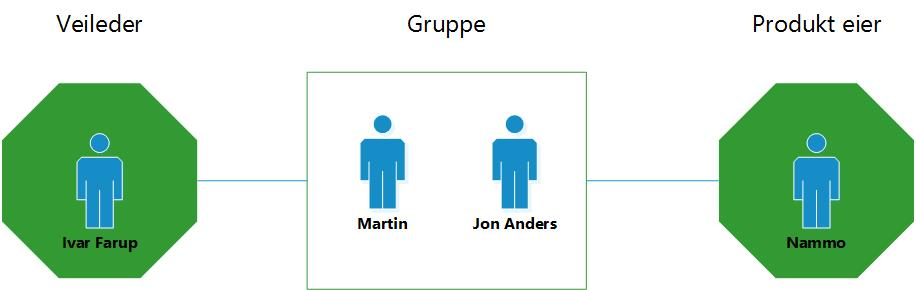
\includegraphics{Scrumroller1}

Figur 1 : Representasjon av scrum rollene


\section{Akademisk bakgrunn}
De siste 3 årene har begge medlemmene studert ved Norges teknisk-naturvitenskapelige universitet. Martin har studert programvareutvikling og Jon anders har studert Data ingeniør. Dette har gjort at vi begge har mye av den samme kunnskapen men i tillegg erfaringer i forskjellige felt. Dette har gitt oss en tyngde i forskjellige programmeringsspråk som C++, java, mysql, php, javascript og andre scriptspråk som bash og powershell. Martin har i tillegg tatt er ergonomi i digitale medier fag. Som fokuserer på brukerinteraksjon med systemet. Jon Anders har erfaring med matte 1 og 2, noe som ble brukt mye under utviklingsprosessen. Den største forskjellen mellom oss har vært mattekunnskapene, den har ført til at Jon Anders ble jobbende hovedsakelig med algoritmen og andre matematiske krevende arbeid. Martin ble jobbende mer med oppgaver som ikke krevde så mye matematiske ferdigheter, som GUI, design rapportskriving og andre funksjonaliteter som eksportering til Excel.



\section{Dokumentstruktur} 

\textbf{Introduksjon}\\
dette kapittelet presenterer prosjektet til leseren, introduserer gruppen, arbeidsgiveren og veilederen, samt generell informasjon om prosjektet\\

\textbf{Prosjektorganisering}\\
Dette kapittelet introduserer leseren til utviklingsprosessen og store avgjørelser som ble tatt tidlig i prosjektet.\\

\textbf{Kravspesifikasjoner}\\
	Dette prosjektet gir en dypere introduksjon til kravspesifikasjonene.\\

\textbf{Teknisk Design}\\
Dette kapittelet gir en oversikt over valget av språk, rammeverk, utviklingsmiljø, hvordan vi har tolket kravspesifikasjonene og arkitektur designet.\\	

\textbf{Implementasjon}\\
Dette kapittelet viser en oversikt over hvordan de viktigste funksjonene har blitt implementert.\\ 

\textbf{Utviklingsprosess}\\
Dette kapittelet gir leseren et innblikk i utviklingsprosessen , hvilke problemer vi har møtt og hvordan vi har valgt å løse dem.\\

\textbf{Testing og Kvalitetssikring}\\
	Dette kapittelet gir et detaljert innblikk i hvordan vi har testet og kvalitetssikret koden.\\

\textbf{Diskusjon}\\
Dette prosjektet inneholder en diskusjon av hele prosjektet, sammenlikning av oppgaven opp mot resultatet. Gruppen sin refleksjon av arbeidet som har blitt gjort og resultatet som har blitt levert.\\

\textbf{Konklusjon}\\
	Dette kapittelet konkluderer kort hele prosjektet og rapporten.\\





  